\chapter{Implementation}
\label{chap:implementation}
This chapter details the technical implementation of the ResNet-BiLSTM-Attention framework \autocite{Fischer2025ResNetBiLSTM} by putting the conceptual framework from \autoref{chap:methodology} into a functional system that processes manufacturing OCEL, extracts relevant features, trains models, and evaluates the fidelity of SBDT.

\section{Architecture and System Setup}

\subsection{Architecture}
The implementation follows a modular architecture. It can process both streams and batches of manufacturing data.

\begin{figure}[htbp]
  \centering
  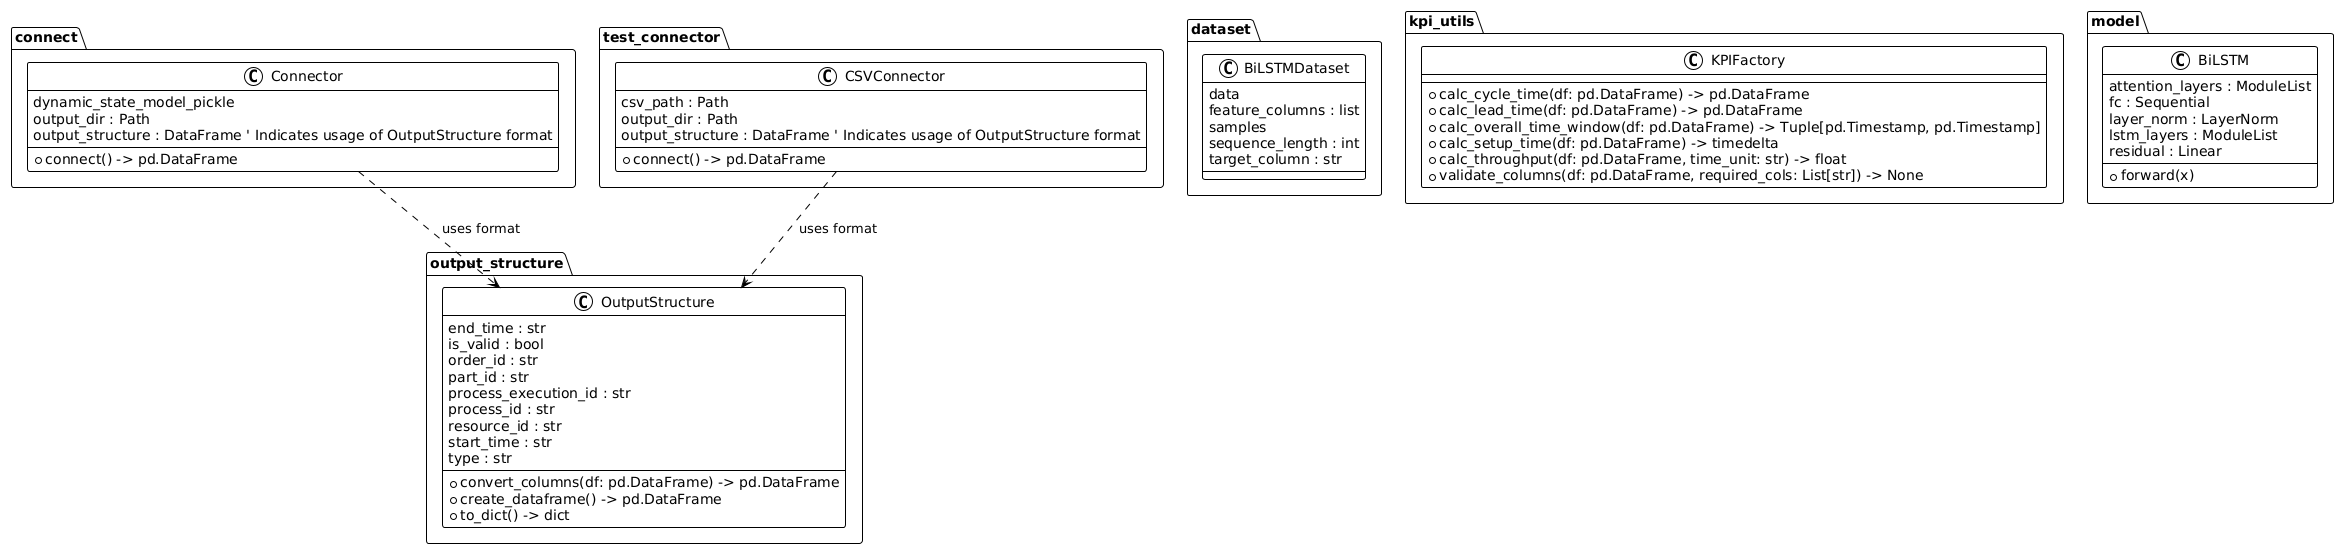
\includegraphics[width=0.8\textwidth]{figures/code.png}
  \caption{Unified Modelling Language (UML) diagram of the ResNet-BiLSTM-Attention framework for validating SBDT in manufacturing environments.}
  \caption*{Source: Own figure.}
  \label{fig:uml-diagram}
\end{figure}

The UML model \autocite{PlantUML} in \autoref{fig:uml-diagram} illustrates the system's architecture, which consists of several components that interact to achieve the validation of SBDT. The components include:
\begin{itemize}
  \item \textbf{Data Connectors:} In the given code, two classes \texttt{InputStructure} and \texttt{OutputStructure} are responsible for reading and writing data. The \texttt{InputStructure} class reads raw data from the twin simulation, while the \texttt{OutputStructure} class writes the processed data into the OCEL format developed for this framework, see \autoref{sec:event_log_processing}. The mapping logic is returned as well. The connector assigns IDs for different parts, resources, and processes. The IDs are used to identify the different components in the manufacturing process. This is a requirement for OCED. The mapping is returned as JSON files for each category, respectively.
  \item \textbf{KPIFactory:} Contains utility functions to calculate a diverse set of KPIs for PPC evaluation of the process.
  \item \textbf{Baseline Model:} Implements a baseline model for comparison with the ResNet-BiLSTM-Attention model. This model serves as a reference point to evaluate the performance of the more complex architecture.
  \item \textbf{PyTorch DataSet and DataLoader:} Handles the conversion of raw data into a format suitable for the ResNet-BiLSTM-Attention model.
  \item \textbf{ResNet-BiLSTM-Attention:} The core model that combines ResNet and BiLSTM architectures with attention mechanisms to learn from the data.
\end{itemize}

\subsection{Tech Stack and Setup}
The implementation is built with Python 3.12 \autocite{Python}, using the following frameworks and libraries:

\begin{itemize}
  \item \textbf{PyTorch:} Powers the deep learning components, chosen for its dynamic computational graph that facilitates complex architecture development and debugging \autocite{PyTorch}.
  \item \textbf{Pandas \& NumPy:} Handle data manipulation, transformation, and numerical operations \autocite{NumPy, Pandas}.
  \item \textbf{Scikit-learn:} Provides implementation of the baseline model and evaluation metrics \autocite{ScikitLearn}.
  \item \textbf{Matplotlib \& Graphviz:} Generate visualizations of model architecture and performance \autocite{Matplotlib, Graphviz}.
  \item \textbf{UV Package Manager:} Ensures reproducible dependency management with exact version pinning \autocite{UV}.
\end{itemize}

Besides well established packages, PyTorch was preferred over TensorFlow due to its flexibility and ease of use, especially for research purposes. The implementation is designed to be modular and extensible, allowing for future enhancements and adaptations to different manufacturing environments.
The system is designed to run on a standard workstation with a multi-core CPU and an optional GPU for accelerated training. The given framework utilizes CUDA \autocite{NVIDIA_CUDA} for GPU acceleration, which significantly speeds up the training process. The system is capable of processing large datasets efficiently, making it suitable for real-time applications in manufacturing environments.


\section{Data Preprocessing}
\label{sec:event_log_processing}

After laying out the architecture and system setup, this section focuses on the data preprocessing steps necessary for preparing the input data for the baseline model.

\subsection{OCEL Format}

Both models used in this thesis require the input data to be in the OCEL format, see \autoref{sec:object-centric-event-logs}. The columns are inspired by the twin comparison model by \autocite{schwede2024learning}. For the given framework, the format is expected as input in the following format:

\begin{table}[htbp]
  \centering
  \caption{Detailed structure, data types, and description of the processed manufacturing OCEL.}
  \label{tab:output_structure_detailed}
  % Adjust the width 'p{6cm}' of the description column as needed, or use tabularx
  \begin{tabular}{l l p{6cm}} % l=left-aligned, p{width}=paragraph column
    \toprule
    \textbf{Column Name}            & \textbf{Data Type}       & \textbf{Description}                                                                                                                              \\
    \midrule
    \texttt{process\_execution\_id} & \texttt{int}             & Unique identifier for the specific process recorded.                                                                                              \\
    \texttt{order\_id}              & \texttt{Index (int/str)} & Identifier for the overall manufacturing order this event belongs to.                                                                             \\
    \texttt{start\_time}            & \texttt{Timestamp [UTC]} & The precise timestamp marking the beginning of the event, adjusted to UTC.                                                                        \\
    \texttt{end\_time}              & \texttt{Timestamp [UTC]} & The precise timestamp marking the end of the event, adjusted to UTC.                                                                              \\
    \texttt{duration}               & \texttt{float} (seconds) & The calculated duration of the event (\texttt{end\_time} - \texttt{start\_time}) in total seconds.                                                \\
    \texttt{part\_id}               & \texttt{int}             & Identifier for the specific part or component being processed or handled during the event.                                                        \\
    \texttt{resource\_id}           & \texttt{int}             & Identifier for the machine, station, or other resource involved in the event.                                                                     \\
    \texttt{process\_id}            & \texttt{int}             & Identifier indicating the type of process step or operation performed (e.g., milling, assembly).                                                  \\
    \texttt{type}                   & \texttt{str}             & A textual description or category classifying the type of event recorded.                                                                         \\
    \texttt{is\_valid}              & \texttt{bool}            & Boolean flag indicating whether the recorded event sequence or outcome is considered valid (e.g., based on model prediction or predefined rules). \\
    \bottomrule
  \end{tabular}
\end{table}

The terms are consistent with the upper cited framework. For the model components, following features may be considered:

\begin{enumerate}
  \item \textbf{Time Model:} \texttt{duration}, \texttt{start\_time}, \texttt{end\_time} and further engineered features.

  \item \textbf{Transition Model:} \texttt{process\_id}, \texttt{resource\_id}, \texttt{end\_time}.

  \item \textbf{Transformation Model:} \texttt{part\_id}.

  \item \textbf{Quality Model:} Exclusion of quality information in the given model.

  \item \textbf{Resource Model:}\texttt{resource\_id}, \texttt{process\_id}, \texttt{part\_id}.

  \item \textbf{Resource Capacity Model:} \texttt{resource\_id}; Note: Insufficient data available for detailed capacity modelling.

  \item \textbf{Process Model:} \texttt{process\_id}, \texttt{part\_id}, \texttt{resource\_id}.
\end{enumerate}

This table does not forbid adding relational logic by the modeller. For example, each ID may be a foreign key to another table. Each row in the OCEL represents a single event instance. This schema aligns with OCED principles (\autoref{sec:object-centric-event-logs}) by explicitly linking each recorded event instance (\texttt{process\_execution\_id} per timestamp) to the multiple object instances (\texttt{order\_id}, \texttt{part\_id}, \texttt{resource\_id}, \texttt{process\_id}) involved in its execution. This inherent multi-object relationship within each event record is important for modelling complex process dependencies. The structure empowers the representation of complex control flows often found in manufacturing. Parallel execution paths (AND-split) can be inferred by identifying events associated with different resources or process steps occurring \textit{within} overlapping time intervals (\texttt{start\_time}, \texttt{end\_time}) but related to shared object instances, such as a common \texttt{order\_id}. Alternative paths and process variants (EXCLUSIVE OR-split) are explicitly captured through the diversity of event sequences observed across different process instantiations (e.g., grouped by \texttt{order\_id}); the log records exactly which path or sequence of activities occurred for each instance. The object-centric nature enriches this analysis by providing context (e.g., the specific \texttt{part\_id} or \texttt{resource\_id} involved) that can explain why a particular variant or choice was executed. The OCEL retains its sequential linear character by grouping it by \texttt{order\_id} and sorting ascending related to \texttt{end\_time}. This allows for the reconstruction of the process flow. The use-case in \autoref{chap:case-study} will engineer further features from the OCEL format.

Because conciseness of the data structure was a requirement, the OCEL format is not fully compliant with the OCED standard \autocite{van2023object}. The OCEL format used in this thesis is rather simplified. Specifically, this simplification means the schema does not include distinct tables for object instances and their types, explicit modelling of static O2O relationships (\autoref{sec:object-centric-event-logs}) or the capability to store timestamped attributes associated directly with objects rather than events. Despite these omissions the implemented structure retains the core OCED principles. The goal is rather to \textit{learn} these relationships from the data itself.

\section{Model Implementation}

After the basic OCEL format is established, the next step is to implement the models. The implementation consists of two main components: a baseline model and the black-box model. The baseline model serves as a reference point for evaluating the performance of the more complex architecture. The ResNet-BiLSTM-Attention model is designed to learn from the data and make predictions based on the features extracted from the OCEL format, as well as the baseline model does. The key distinction lies in interpretability: while the DT baseline (white-box) enables direct rule extraction, the ResNet-BiLSTM-Attention (black-box) trades explainability for sequential pattern capture. In the course of the experiments, the baseline model can serve as a VVUQ tool by itself. Data leakage may be diagnosable by analysing the results of the \texttt{DecisionTreeClassifier}. Furthermore, model components can be analysed by themselves through adaptive feature selection during training. If the classifier was able to learn well on the dataset, the model component may be present in the dataset and thus the SBDT was able to encode this information in the data. The ResNet-BiLSTM-Attention model is a black-box model, which means that the decision-making process is not easily interpretable. The \texttt{DecisionTreeClassifier} will thus from now on often be referred to as 'white-box model' or 'baseline model'. The ResNet-BiLSTM-Attention model will be referred to as 'black-box model'. The implementation of both models is described in detail in the following sections.

The general modelling decision is as follows: The models receive a binary classification task. The task is to predict whether the process execution is 'valid' or not. Validity in the sense is also including verification and uncertainty quantification. If the row or process is not valid ('accurate'), the modeller has to further identify the root cause. The models thus serve as a diagnostic tool to conduct more deep analysis. UQ is achieved by measuring the metrics of both models. Verification is achieved by the manual efforts of the modeller\footnote{Of course, this undermines our efforts to present a fully automatic VVUQ framework. A lot of time is saved in the timespan when no validity breach is detected. This is the main advantage of this approach.}. The \texttt{is\_valid} column in the OCEL format serves as the target variable. The models are trained on a subset of the data, and their performance is evaluated on a separate test set. The models are compared based on various metrics, including accuracy, precision, recall, and F1-score. The goal is to determine which model performs better in terms of predicting the validity of process executions. Both models are compared using the same metrics described in \autoref{sec:metrics-theory}. The models are trained and evaluated using the same dataset, ensuring a fair comparison. The results are presented in \autoref{chap:case-study}. The data has been sorted by \texttt{end\_time} and grouped by \texttt{order\_id} to ensure that the white-box model has a chance to learn sequential patterns as well. By nature, decision tree classifiers are not able to learn sequential patterns. The ResNet-BiLSTM-Attention model is able to. For the train-test split, a random split is used. Despite sequential nature, random splitting was prioritized to mitigate temporal bias from incomplete process traces \autocite{morita2022investigation}. Temporal bias refers to wrongly guessed correctness of patterns which are induced by choosing wrong cut-off points for splits.


\subsection{Whitebox Baseline Model}
As a baseline model, a white-box model is implemented to provide a reference point for the performance of the ResNet-BiLSTM-Attention model. The white-box model is based on a simple decision tree classifier, which is interpretable and easy to understand. This model serves as a benchmark for evaluating the performance of the more complex ResNet-BiLSTM-Attention model. For the concrete implementation, the \texttt{DecisionTreeClassifier} from the \texttt{sklearn.tree} module is used \autocite{ScikitLearn}.

\subsection{ResNet BiLSTM Multi-Head Self-Attention Network}
As a primary 'challenger' model, the ResNet-BiLSTM-Attention model is implemented, see \autoref{sec:integrated_architecture}. This model combines the strengths of residual networks (ResNet) and bidirectional long short-term memory networks (BiLSTM) with multi-head self-attention mechanisms. The model is implemented using the PyTorch modules \texttt{torch.nn}, \texttt{torch.functional} and \texttt{torch.optim} \autocite{PyTorch}. Before the data is ingested by the network, specific \texttt{DataSet} and \texttt{DataLoader} classes are implemented to handle the data. The \texttt{DataSet} class is responsible for loading the data and transforming it into a format suitable for the model. The \texttt{DataLoader} class is responsible for batching the data and shuffling it during training.

\begin{figure}[htbp]
  \centering
  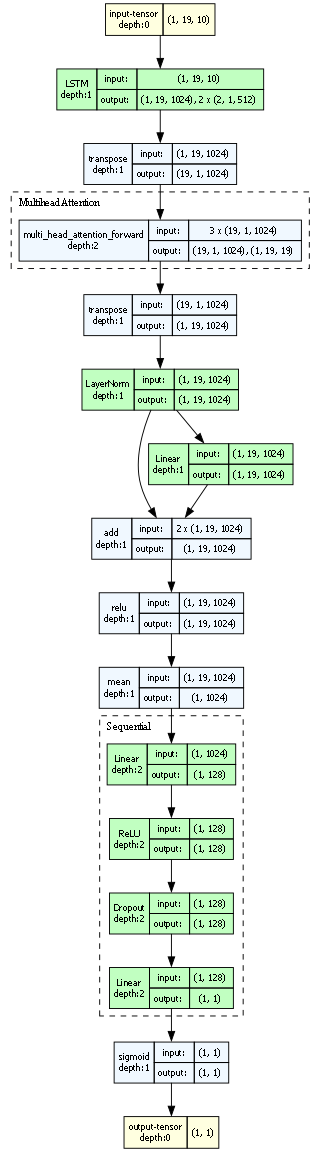
\includegraphics[width=0.4\textwidth]{figures/architecture.png}
  \caption{ResNet-BiLSTM-Attention architecture. The model consists of a ResNet block, followed by a BiLSTM layer and a multi-head self-attention mechanism. The output is then passed through a fully connected layer for classification.}
  \label{fig:architecture}
  \caption*{Source: Own Torchview illustration.}
\end{figure}

The architecture of the ResNet-BiLSTM-Attention model is shown in \autoref{fig:architecture}. The \texttt{torch.nn} module integrates Bidirectional Long Short-Term Memory (BiLSTM) layers with Multi-Head Self-Attention and Residual Connections. The model architecture consists of several layers, including convolutional layers, BiLSTM layers, and attention mechanisms.

\begin{enumerate}
  \item \textbf{Input/Configuration:} The model is initialized with hyperparameters defining its structure: \texttt{input\_size} (number of input features, $D$), \texttt{hidden\_size} (dimensionality of LSTM states, $H$), \texttt{num\_layers} (number of stacked LSTM/Attention blocks, $N$), and \texttt{attention\_heads} (number of parallel attention heads, $A$).

  \item \textbf{BiLSTM Layers:} The core consists of $N$ stacked BiLSTM layers (\texttt{nn.LSTM} with \texttt{bidirectional=True}). Each layer processes the input sequence in both forward and backward directions, capturing dependencies from past and future context. The output dimensionality of each BiLSTM layer is $2H$. Dropout is applied between layers for regularization.

  \item \textbf{Multi-Head Self-Attention:} Following each BiLSTM layer, a \texttt{nn.MultiheadAttention} layer is applied. It performs self-attention on the BiLSTM output sequence, allowing the model to weigh the importance of different time steps relative to each other within the sequence.

  \item \textbf{Layer Normalization \& Residual Connections:} \texttt{nn.LayerNorm} is applied after the attention mechanism within each block to stabilize activations. A residual connection adds the input to this block to the output before a final \texttt{ReLU} activation, facilitating gradient flow in deeper networks.

  \item \textbf{Sequence Pooling:} After the final LSTM/Attention block, the output sequence (shape: $Batch \times Sequence Length \times 2H$) is aggregated across the sequence dimension using temporal mean pooling (\texttt{torch.mean}), resulting in a single fixed-size vector (shape: $Batch \times 2H$) representing each input sequence.

  \item \textbf{Final Classifier:} A feed-forward network (\texttt{nn.Sequential}) processes the pooled representation. It typically includes one or more linear layers with \texttt{ReLU} activations and Dropout for regularization, culminating in a final linear layer producing a single output logit.

  \item \textbf{Output Activation:} A sigmoid function (\texttt{torch.sigmoid}) is applied to the final logit to produce a probability score between 0 and 1, suitable for binary classification.

  \item \textbf{Weight Initialization:} Linear layers within the network are initialized using Kaiming Normal initialization (\texttt{nn.init.kaiming\_normal\_}), a standard practice often beneficial for layers followed by \texttt{ReLU} activations.
\end{enumerate}

For training, the model has to be set to inference mode using the \texttt{train\_model()} method. The model is trained using the Adam optimizer \texttt{torch.optim.Adam} \autoref{eq:adam,eq:adam_update} \autocite{kingma2014adam} to update model weights based on calculated gradients. The loss function used is binary cross-entropy \autoref{eq:bce} \texttt{nn.BCELoss}. It quantifies the difference between the predicted probabilities and the true binary labels. The learning rate is not fixed, rather a learning rate scheduler \texttt{torch.optim.lr\_scheduler.ReduceLROnPlateau} is used to adjust the learning rate during training based on the performance on a monitored metric (e.g., training or validation loss). The model is trained for a specified number of epochs, and the training loop iterates over the training dataset in mini-batches. In each epoch, the model performs forward and backward passes to compute loss and gradients, updating model parameters using the optimizer. Training loss is typically tracked per epoch.

\section{Model Evaluation}
Based on the reference in \autoref{sec:metrics-theory}, the evaluation of the models is performed using various metrics. To achieve this, the model is switched to evaluation mode, \texttt{model.eval()}, to ensure deterministic behaviour. This disables dropout layers so that all neurons are used for the forward pass to achieve predictions. Gradient calculations are disabled through \texttt{torch.no\_grad()}. \texttt{BatchNorm} layers now use their learned estimates of mean and variance parameters to process the data. During evaluation mode, the model processes the test set batch per batch, yielding output probabilities. These are compared against the true labels. The evaluation metrics are implemented in the \texttt{evaluate\_model()} method. The evaluation metrics include a classification report, confusion matrix \autoref{tab:confusionmatrix}, accuracy \autoref{eq:accuracy}, precision \autoref{eq:precision}, recall \autoref{eq:recall}, F1-score \autoref{eq:F1-score} and ROC AUC score \autoref{eq:auc}. The metrics are calculated using the \texttt{sklearn.metrics} module. The evaluation metrics are used to compare the performance of the baseline model and the ResNet-BiLSTM-Attention model as well as the standalone performance on the holdout set. The evaluation metrics are also used to diagnose the models and identify potential issues with respect to the bespoken adaptive feature selection procedure. For the assignment of the label 'valid' or 'invalid', a threshold of $0.9$ is used. This value is higher than the usual threshold of $0.5$. This means that if the predicted probability is greater than or equal to $0.9$, the process execution is classified as 'valid'. If the predicted probability is less than $0.9$, the process execution is classified as 'invalid'. Setting the boundary so high is a conservative approach. It ensures that only the most confident predictions are classified as 'valid'. This is important for the VVUQ framework, as it aims to identify potential issues in the process execution. The threshold can be adjusted based on the specific requirements of the application and the desired trade-off between precision and recall. The $0.9$ validity threshold reflects manufacturing VVUQ's low tolerance for false positives \autoref{eq:precision}.

The evaluation logic presented so far applies to batch data. The idea of the black-box model and concurrent VVUQ lies in processing stream data, preferably in chunks equal to the \texttt{sequence\_length} of one batch of the network during the evaluation phase. Pandas \autocite{Pandas} provides the \texttt{chunksize} parameter to read the data in chunks. The \texttt{chunksize} parameter can be set to the \texttt{sequence\_length} of the model. The model is then evaluated on each chunk of data. The evaluation metrics are calculated for each chunk updated in real time for PPC and direct reporting. This can be applied on the white-box model as well. For the black-box model, this implementation may be achieved using specific \texttt{DataLoader} classes. For concurrent evaluation, UCL and LCL can be set. If they are exceeded, the model will raise an alert. This approach is inspired by the p-chart approach used by \autocite{dos2024simulation}.

If desired, the learned parameters of the model can be saved to a file using the \texttt{torch.save()} method. This allows the trained model to be loaded later for inference or further analysis without repeating the training process. The model can be saved in two different formats: the entire model or just the state dictionary. The state dictionary contains all the parameters of the model, while the entire model includes the architecture and parameters. The state dictionary is preferred for saving models, as it is more flexible and allows for easier loading of models with different architectures.